
% \begin{frame}{Future work}

% How do you peform model checking with sensitivity analysis?

% Existing methods evaluate whether the analysis changes ``a lot'' when you:
% %
% \begin{itemize}
% \item Parametrically perturb the model (e.g.~fit a richer model class)
% \item Non--parameterically perturb the data (e.g.~produce gross outliers)
% \end{itemize}
% %
% The problem is:
% %
% \begin{itemize}
% \item How much is ``a lot''?
% \item Non--parametric data perturbations are hard to reason about
% \item It's hard to say whether parametric model changes are enough
% \end{itemize}
% %


% Instead, we
% %
% \begin{itemize}
% \item Parametrically perturb the data
% \item Observe whether our model could detect the change
% \end{itemize}
% %
% \begin{itemize}
% \item Know exactly the expected change (don't have to decide on what ``a lot'' means)
% \item Easy to reason about whether the data perturbation is reasonable
% \item Don't need to propose an alternative model, instead study the model you have
% \end{itemize}


% \end{frame}

\begin{frame}{Related and future work}

Today, I focused on covariate balance.  In this work, we also provide rigorous justification for
%
\begin{itemize}
\item Frequentist covariance estimation
\item Parital pooling
\item Negative weights (extrapolation)
\end{itemize}
%
\pause
\textbf{Student contributions and future work:}

\begin{itemize}
\item \textbf{Alice Cima} contributed significantly to this work
\item \textbf{Vladimir Palmin} is working on extending MrPlew to \texttt{lme4}
\item \textbf{Sequoia Andrade} is working on generalizing to other local sensitivity checks
\item \textbf{Lucas Schwengber} is working on novel flow--based techniques for local sensitivity
\end{itemize}


\begin{minipage}[t]{0.24\textwidth}
    \centering
    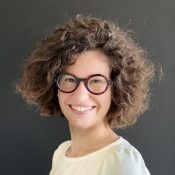
\includegraphics[width=0.9\textwidth]{static_figures/alice.jpg}\\
    Alice Cima
\end{minipage}
\begin{minipage}[t]{0.24\textwidth}
    \centering
    No picture!\\
    Vladimir Palmin
\end{minipage}
\begin{minipage}[t]{0.24\textwidth}
    \centering
    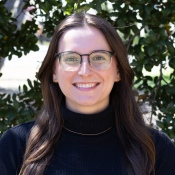
\includegraphics[width=0.9\textwidth]{static_figures/sequoia.jpg}\\
    Sequoia Andrade
\end{minipage}
\begin{minipage}[t]{0.24\textwidth}
    \centering
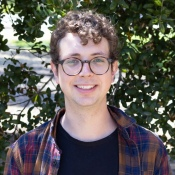
\includegraphics[width=0.9\textwidth]{static_figures/lucas.jpg}\\
Lucas Schwengber
\end{minipage}

\end{frame}

%%%%%%%%%%%%%%%%%%%%%%%%%%%%%%%%%%%%%%%%
%%%%%%%%%%%%%%%%%%%%%%%%%%%%%%%%%%%%%%%%
%%%%%%%%%%%%%%%%%%%%%%%%%%%%%%%%%%%%%%%%


